\documentclass[11pt]{article}
\usepackage{hyperref}
\usepackage[english]{babel}
\usepackage{blindtext}
\usepackage{url}
\usepackage{graphicx}
\usepackage{multicol}
\usepackage[center]{titlesec}
\usepackage{geometry}
\usepackage{lettrine} % The lettrine is the first enlarged letter at the beginning of the text

%\usepackage{mathtools}

\usepackage[sort, numbers]{natbib}


%
%\setlength{\columnseprule}{0.4pt}
%\setlength{\footskip}{20pt}
\usepackage{fancyhdr}
\fancyhf{}
\fancyhead[C]{PHC 7000 $\bullet$ Joe Brew $\bullet$ HW 5}
%\fancyfoot[C]{  $\bullet$ Sample Size \bullet$  }
\renewcommand\headrulewidth{1pt}
\renewcommand\footrulewidth{1pt}
\pagestyle{fancy}

%

\setlength{\columnsep}{1.5cm}
%\setlength{\columnseprule}{0.4pt}

%\MakeOuterQuote{"}



\graphicspath{ {"C:/Users/BrewJR/Documents/uf/phc7000/hw5/hw5_brew} }

%the next two lines adjust the third, centered section of the exec sum
\def\changemargin#1#2{\list{}{\rightmargin#2\leftmargin#1}\item[]}
\let\endchangemargin=\endlist 

\usepackage{Sweave}
\begin{document}
\Sconcordance{concordance:hw5_brew.tex:hw5_brew.Rnw:%
1 42 1 1 0 55 1 1 7 1 2 11 1 1 19 1 2 55 1}


\title{\textbf{Homework 5: Program Evaluation}}
\author{Joe Brew}


\maketitle

\emph{\begin{center} 
joebrew@gmail.com \\ 
UFID: 0402-8902 \\ 
+001 352 318 4553 \\ 
\end{center}}

\tableofcontents

\vspace{20mm}

\begin{center}

\includegraphics[width=2cm]{uf}
\end{center}


\newgeometry{margin=3.5cm}
%\fancyhfoffset[E,O]{0pt}


%------------------------------------------
\section*{Homework 5: Program evaluation}
\addcontentsline{toc}{section}{Homework 5: Program evaluation}
%------------------------------------------
\hrulefill

\begin{multicols}{2} 
\setkeys{Gin}{width=0.45\textwidth}

%------------------------------------------
\subsection*{0. My chapter: Justify Conclusions}
\addcontentsline{toc}{subsection}{0. My chapter: Justify Conclusions}
%------------------------------------------
\lettrine[nindent=0em,lines=3]{S}{tep five} of the CDC manual on program evaluation involves analysis of evidence and conclusion-making from that analysis, with the end of "justifying the claims by comparing the evidence against stakeholder values." \cite{cdc}. The chapter outlines the challenges (particularly the fact that different stakeholders may have different values by which to measure "effectiveness") and methods best suited for analysis and conclusion-making. \\

The CDC recommends that stakeholders must "articulate" their values \emph{a priori}, so that an objective comparison between those values and the program evaluation's results can be made.  They gave a rather basic overview of what to remember when interpreting findings (pertinence, bias, alternative explanations, consistency, validity, etc.), and provide a basic checklist to help those conducting a program evaluation be sure that their results are valid and adequately address stakeholders' values.

%------------------------------------------
\subsection*{1. Definition}
\addcontentsline{toc}{subsection}{1. Definition}
%------------------------------------------
\emph{Define program evaluation in your own words. (1 -2 sentences).}\\

\lettrine[nindent=0em,lines=3]{P}{rogram evaluation} is essentially the comparison of a program's stated aims (values, goals, etc.) with its results or impact.  The more closely these two metrics coincide (aim and impact), the more favorably a program can be evaluated. \\

Below is a visual representation of how a program can be evaluated, with point size corresponding to evaluation (ie, big points = good program).  Lofty aims (x-axis) and high impact results (y-axis) are not "rewarded" in evaluation unless they coincide (diagonal line).

\begin{center}
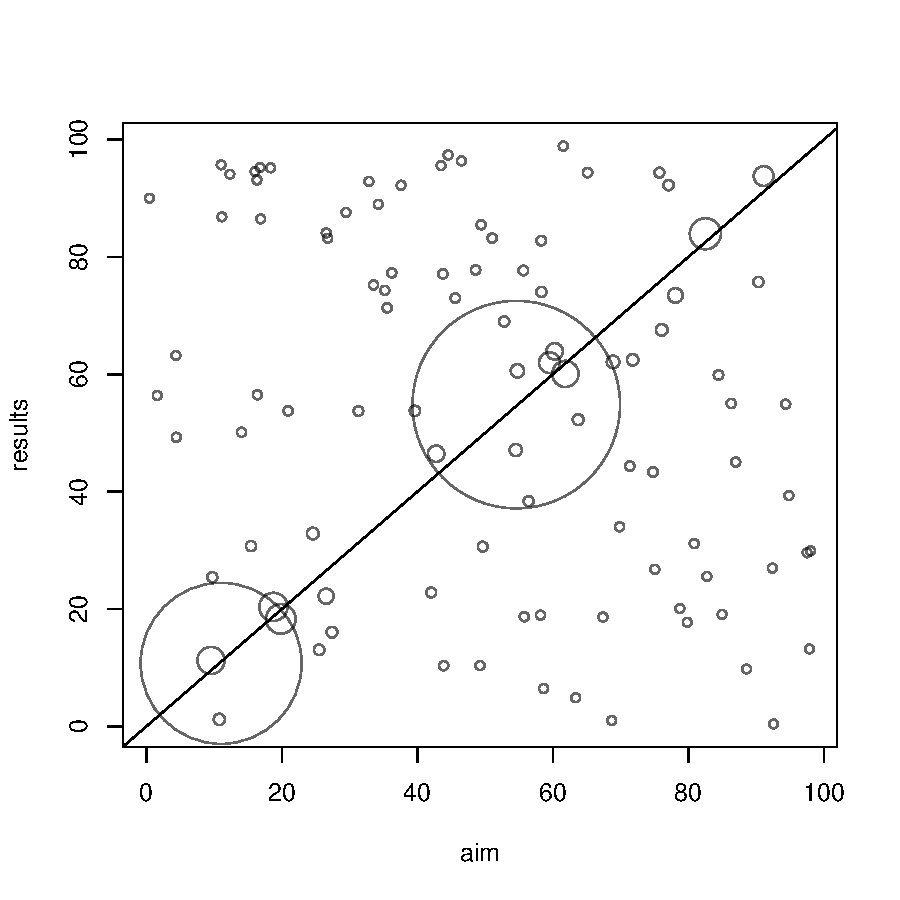
\includegraphics{hw5_brew-001}
\end{center}

%------------------------------------------
\subsection*{2. Difference between program evaluation and epidemiological research}
\addcontentsline{toc}{subsection}{2. Difference between program evaluation and epidemiological research}
%------------------------------------------
\emph{What do you think is the main difference between program evaluation and epidemiological research?} \\
\lettrine[nindent=0em,lines=3]{W}{hereas} epidemiological research deals with questions of theoretical truth and generalizability, program evaluation deals more in the merits of a specific program.  While epidemiology and program evaluation use many of the same methods, their purposes differ: epidemiology wants to draw insights and make conclusions which are externally valid and generalizable to populations on the whole; program evaluation is more concerned with operational integrity and practicality, and how best to measure the specific impact of operations so as to improve them.  \\

To qualify the above statement, I think there is more overlap than most "program evaluators" or epidemiologists would care to admit (see below). Many times, "research" is simply evaluation of a program (or collection of programs), and program evaluation often implies generalizability.  

\begin{center}
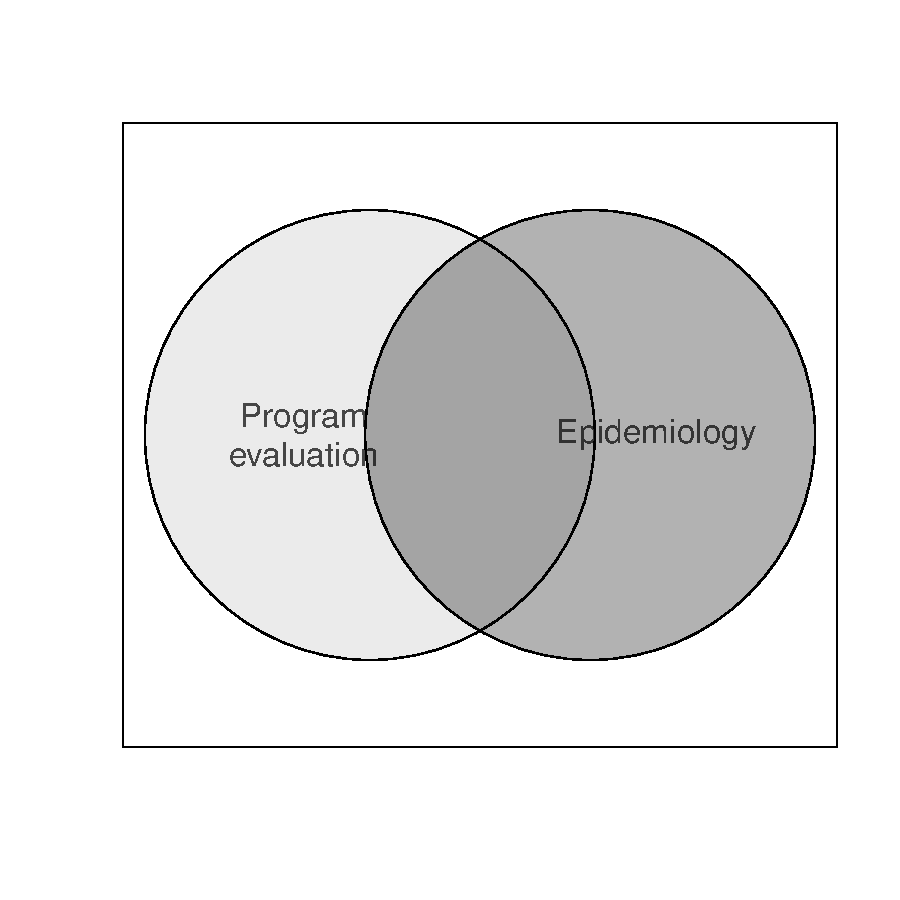
\includegraphics{hw5_brew-002}
\end{center}
%------------------------------------------
\subsection*{3. Rotavirus paper}
\addcontentsline{toc}{subsection}{3. Rotavirus paper}
%------------------------------------------

\emph{Based on the paper "Effectiveness of the monovalent rotavirus vaccine in Colombia: A case-control study", Do you think they apply the step that you read in the CDC guideline? How can they improve the rotavirus evaluation next time?}

\lettrine[nindent=0em,lines=3]{I}{n} Cotes-Cantillo et al's paper on rotavirus vaccine in Colombia, I believe that the authors did a very good job applying the CDC's 5th step of program evaluation (justify conclusions) to their analysis.\cite{CotesCantillo2014}  They sought to assess the effectiveness of the vaccine, defined how they would assess effectiveness (ie, clarification of values), demonstrated quantiatively that effectiveness, addressed the potential issues of bias, confounding and validity (discussion on caveats, page 3039, second column), and were transparent about the processes and methods which led them to their conclusion.

%------------------------------------------
\subsection*{4. Additional assignment}
\addcontentsline{toc}{subsection}{4. Additional assignment}
%------------------------------------------

Here is an additional assignment related to reviewing for journals, that should take no more than about 30 minutes:

Read the "reviewer guidelines" for Elsevier, a publisher of several major medical and public health journals.  \footnote{\href{http://www.elsevier.com/reviewers/reviewer-guidelines\#conducting-a-review}{http://www.elsevier.com/reviewers/reviewer-guidelines\#conducting-a-review}   } 



\textbf{1.  Note that one of the issues is related to ethics.  Click on the ethics link and look at the ethical issues related to researchers.  Name 3-4 of the most important ethical issues that can come up when reviewing papers.} 

The most important ethical issues that can come up when reviewing papers are plagiarism, fraud and undisclosed conflicts of interest.\footnote{\href{http://www.elsevier.com/editors/perk}{http://www.elsevier.com/editors/perk}}

\textbf{2.   Read about what the journal is looking for within each section of a manuscript.  Under the "methods" click on the link to the most common statistical errors.\footnote{\href{http://www.elsevier.com/\_\_data/assets/pdf\_file/0008/110996/reviewers\_statistics.pdf}{http://www.elsevier.com/\_\_data/assets/pdf\_file/0008/110996/reviewers\_statistics.pdf}  } Read this 1-page document for the publisher's recommendations about common statistical issues.  Identify whether there are any that you don't agree with, or state that you agree with all of them.    
}

I don't agree that "dichotomizing continuous variables in the analysis" is only "acceptable for descriptive purposes."  If dichotomization is based on a biologically or otherwise methdologically sound principle, it is perfectly acceptable.  For example, dichotomizing income may be relevant if the study has to do with government benefits that one may receive at a certain income cut-off.  Likewise, dichotomizing blood lead levels may be relevant when either chemically or clinically, a "cut-off" exists or entails different treatments. \\

I also disagree with the guidelines' opposition to multiple testing.  It is true that one can go significance-hunting through multiple tests, but the lack of a clear hypothesis-test-conslusion sequence does \emph{not} mean that a correlation revealed through multiple testing is necessarily value-less.


\end{multicols}
\setkeys{Gin}{width=1\textwidth}
%----------------------------------------------------------------------------------------
%  REFERENCE LIST
%----------------------------------------------------------------------------------------
%\newpage
\bibliographystyle{unsrtnat}
\bibliography{bibliography}

%------------------------------------------
\section*{Details}
\addcontentsline{toc}{section}{Details}
%------------------------------------------
%\hrulefill
%\vspace{10mm}

Full code at \href{https://github.com/joebrew/uf/tree/master/phc7000}{https://github.com/joebrew/uf/tree/master/phc7000}. \\

This report was generated on \today.  The author used R version 3.1.2 (2014-10-31) (Pumpkin Helmet) on a linux-gnu OS.  \\

The analysis in this report was written in the R programming language, and the report production was programmed in \LaTeX{} using Sweave.\\

\end{document}
